\documentclass{beamer}
\usepackage{graphicx}
\usetheme{Warsaw}
\title[]{EE1390}
\subtitle{Matrix Project}
\author{EE18BTECH11016 and EE18BTECH11025}
\date{}
\usepackage{tikz}
\usepackage{tkz-euclide} % loads  TikZ and tkz-base
\usetkzobj{all}
\graphicspath{ {Home/Downloads/} }
\begin{document}


\begin{frame}
\titlepage
\end{frame}

\begin{frame}{Question}

Two sides of a rhombus are along the lines


\setlength{\parindent}{4cm} 
		(7 -1)$\boldsymbol{x}-5=0$


		(1 -1)$\boldsymbol{x}+1=0$
		
		
\setlength{\parindent}{0cm} 
If its diagonals intersect at $\binom{-1}{-2}$, find its vertices.


\setlength{\parindent}{2cm}
[JEE(main) 2016, Q.no. 13 (code G)]
\end{frame}

 


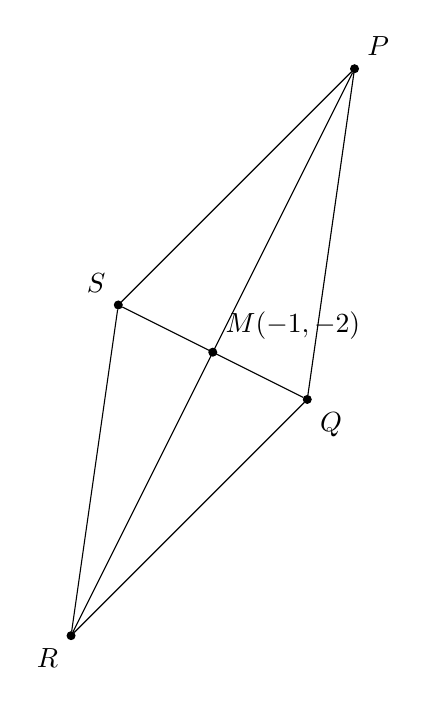
\begin{tikzpicture}
[
 scale=0.9,
  >=stealth,
  point/.style = {draw, circle, fill = black, inner sep = 1pt},
]

\node (P) at (1,2) [point,label = above right:$P{}$] {};
\node (Q) at ( 0.33333333,-2.66666667)[point,label = below right:$Q{}$] {};
\node (R) at (-3,-6)[point,label = below left:$R{}$] {};
\node (S) at (-2.33333333,-1.33333333)[point,label = above left:$S{}$] {};
\node (M) at (-1,-2)[point,label = above right:$M{(-1,-2)}$] {};

\draw (P) -- (Q) -- (R) -- (S) -- (P) -- (R) -- (S) -- (Q);



\end{tikzpicture}




\begin{frame}{Solution}
Given the equations of two lines PQ and PS are :
\setlength{\parindent}{4cm}  

     
 (7 -1)$\boldsymbol{x}-5=0$

		    (1 -1)$\boldsymbol{x}+1=0$
\setlength{\parindent}{0cm}

Solving these two equations , we get the point of intersection as P.
\vspace{2 mm}
\setlength{\parindent}{4cm}

$\binom{7 \ -1}{1  \  -1}$ $\boldsymbol{x}$ = $\binom{5}{-1}$

\vspace{2 mm}
$\boldsymbol{x}$ =  $\binom{1/6 \  -1/6}{1/6  \   -7/6}$ $\binom{5}{-1}$

\vspace{2 mm}

$\boldsymbol{x}$ = $\binom{1}{2}$

\vspace{2 mm}
\setlength{\parindent}{0.5cm}

So coordinates of P in matrix form are $\binom{1}{2}$
\end{frame}

\begin{frame}
Now to find coordinates of point R in matrix form, we need to use the mid-point formula.

Hence,

\setlength{\parindent}{3.6cm}
 M = (P+R)/2
\vspace{2 mm}

\setlength{\parindent}{2cm}
 where M = point of intersection of diagonals
\vspace{2 mm}

\setlength{\parindent}{3.4cm}
 = $\binom{-1}{-2}$

\setlength{\parindent}{3.4cm}
\vspace{2 mm}
R = 2M - P


\vspace{2 mm}
R = $\binom{-3}{-6}$


\vspace{2 mm}

\setlength{\parindent}{0cm}
The direction vector of PR is $\binom{2}{4}$
\vspace{2 mm}
So, normal vector of PR is $\binom{-4}{2}$

\vspace{2 mm}
The equation of QS is (2  4)($\boldsymbol{x}$  -  $\binom{-1}{-2}$) = 0

\vspace{2 mm}
\setlength{\parindent}{4cm}
(2  4)$\boldsymbol{x}$  +  10 = 0

\end{frame}

\begin{frame}
We can get the points Q by finding the intersection of PQ and QS;

\vspace{2 mm}
\setlength{\parindent}{4cm}
(7  -1) $\boldsymbol{x}-5=0$
\vspace{2 mm}

(2   4) $\boldsymbol{x}$  +  10 = 0

\vspace{2 mm}
$\binom{7 \ -1}{2  \   4}$ $\boldsymbol{x}$ = $\binom{5}{-10}$

\vspace{2 mm}
$\boldsymbol{x}$ = $\binom{4/30 \ 1/30}{-2/30  \  7/30}$ $\binom{5}{-10}$


\vspace{2 mm}
Q = $\binom{1/3}{-8/3}$
\end{frame}
 
 
 \begin{frame}
 Similarly for getting S, we find intersection of PS and QS
 
 
 \setlength{\parindent}{4cm}
 
\vspace{2 mm}
 (1  -1) $\boldsymbol{x}+1=0$


\vspace{2 mm}
(2   4) $\boldsymbol{x}$  +  10 = 0


\vspace{2 mm}
$\binom{1 \ -1}{2  \  4}$ $\boldsymbol{x}$ = $\binom{-1}{-10}$


\vspace{2 mm}
$\boldsymbol{x}$ = $\binom{4/6 \ 1/6}{-2/6  \  1/6}$ $\binom{-1}{-10}$

\vspace{2 mm}
S = $\binom{-7/3}{-4/3}$
 \end{frame}



\begin{tikzpicture}
[
 scale=0.9,
  >=stealth,
  point/.style = {draw, circle, fill = black, inner sep = 1pt},
]

\node (P) at (1,2) [point,label = above right:$P{(1,2)}$] {};
\node (Q) at ( 0.33333333,-2.66666667)[point,label = below right:$Q{( 0.334,-2.667)}$] {};
\node (R) at (-3,-6)[point,label = below left:$R{(-3,-6)}$] {};
\node (S) at (-2.33333333,-1.33333333)[point,label = above left:$S{(-2.334,-1.334)}$] {};
\node (M) at (-1,-2)[point,label = above right:$M{(-1,-2)}$] {};

\draw (P) -- (Q) -- (R) -- (S) -- (P) -- (R) -- (S) -- (Q);



\end{tikzpicture}

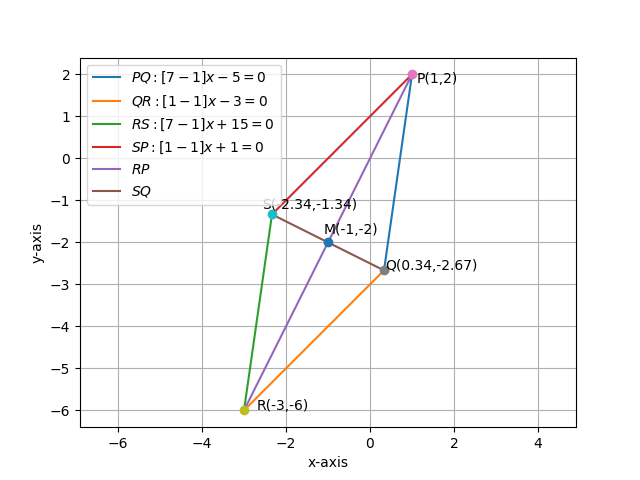
\includegraphics[scale=0.7]{Figure_1.png}

\end{document}
